\documentclass{beamer} % define que é uma apresentação

\usepackage[utf8]{inputenc} % use UTF-8 encode
\usepackage[brazil]{babel} % define a linguagem para português do Brasil
\usepackage{fourier} % use fourier font
\usepackage{ragged2e} % usado para alinhamento de texto

\usepackage[most]{tcolorbox} % permite textos transparentes
\newtcbox{\opacitybox}{blank, on line, opacitytext=0.3} % componente customizado (\opacitybox) que deixa o texto transparente

%% Define o tema da apresentação
\usepackage{themes/beamerthemeAmsterdam} % use Amsterdam theme
% \usetheme{Madrid} % use Madrid theme
% \usecolortheme{default} % use default colors for theme

% \setbeamertemplate{headline} % remove topbar
% \setbeamertemplate{footline} % remove footbar

% remove os símbolos no final da página
\setbeamertemplate{navigation symbols}{}

% define numeração da página em cada slide
\addtobeamertemplate{navigation symbols}{}{
    \usebeamerfont{footline}
    \usebeamercolor[fg]{footline}
    \hspace{1em}
    \insertframenumber
}
\setbeamercolor{footline}{fg=blue}
\setbeamerfont{footline}{series=\bfseries}

% Informações da página de título da apresentação
\title[TCC - Alpha Restful]{Desenvolvimento e Aplicação de um Framework para Otimizações na Implementação de Funcionalidades Sobre Dados Normalizados no MongoDB}

\author[Emanuel Moraes - IFCE - Ciência da Computação]{
    \textbf{Emanuel Moraes de Almeida}\\
    Orientador: Prof. Me. Diego Rocha Lima\\
    Coorientador: Prof. Esp. Thiago Felippe de Lima Bandeira
}

\institute{
    \vspace*{-0.5cm}
    \begin{columns}
        \column{0.9\textwidth}
        \centering{
            \hspace{0.2\textwidth}
            Bacharelado em Ciência da Computação \\
            \hspace{0.2\textwidth}
            Instituto Federal de Educação, Ciência e Tecnologia do Ceará \\
            \hspace{0.2\textwidth}
            IFCE, Brasil, Aracati
        }
        
        \column{0.1\textwidth}
        \vspace{0.5cm}
        \centering{
            
\includegraphics[height=1.5cm]{imagens/ifce-ceara.png}
        }
    \end{columns}
    \vspace*{-0.7cm}
}

\date[IFCE \the\year{}]{
    \today
}

% \logo{
\includegraphics[height=1.5cm]{imagens/ifce-ceara.png}}

% Define o sumário
\AtBeginSection[]
{
    \begingroup
    \setbeamertemplate{navigation symbols}{}
    \begin{frame}
        \frametitle{Sumário}
        \tableofcontents[currentsection]
    \end{frame}
    \endgroup
}

\newcommand{\rmsection}[1]{%
  \par\refstepcounter{section}% Increase section counter
%   \sectionmark{#1}% Add section mark (header)
%   \addcontentsline{toc}{section}{\protect\numberline{\thesection}#1}% Add section to ToC
  % Add more content here, if needed.
}

\begin{document}

\begingroup
\setbeamertemplate{headline}{}
\setbeamertemplate{navigation symbols}{}
\frame{
    \vspace*{-0.5cm}
    \titlepage
} % Cria página de título
\endgroup

\begingroup
\setbeamertemplate{navigation symbols}{}
\begin{frame}
    \frametitle{Sumário}
    \tableofcontents
\end{frame}
\endgroup

\section{Contextualização}

\begin{frame}{Banco de Dados}
    \vspace{1cm}

    \begin{center}
        \begin{minipage}{0.7\linewidth}
            \justifying{``...um sistema cujo objetivo global é registrar e manter informação''}
            \vspace*{-0.3cm}
            \flushright{\scriptsize{(DATE, 2004)}}
        \end{minipage}
    \end{center}
    
    \vspace{0.5cm}
    
    \begin{figure}
        \flushright{
            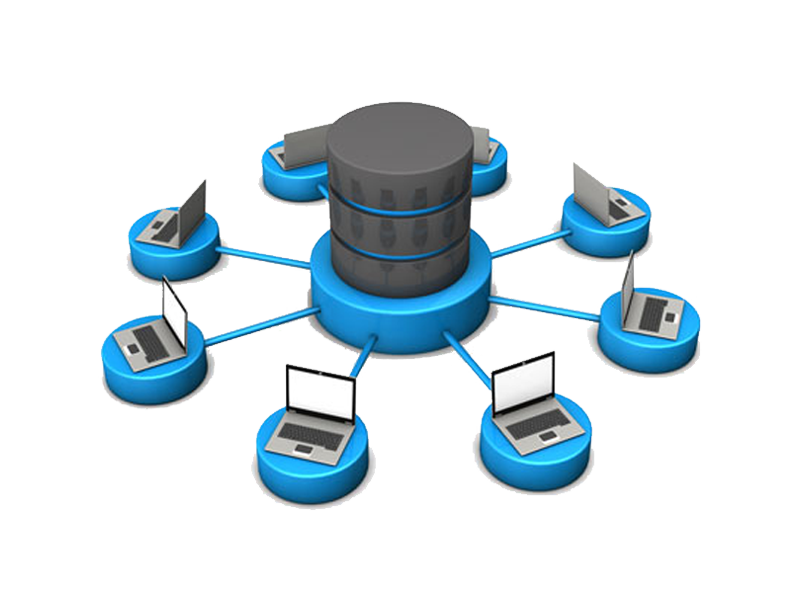
\includegraphics[width=0.5\linewidth]{imagens/banco.png}
            \label{fig:banco-de-dados}
        }
    \end{figure}
\end{frame}

% \begin{frame}{Banco de Dados}
% \begin{columns}
%     \column{0.5\textwidth}

%     “...um sistema cujo objetivo global é registrar e manter informação” (DATE, 2004)
    
%     \column{0.6\textwidth}
    
%     \begin{figure}
%         \centering
%         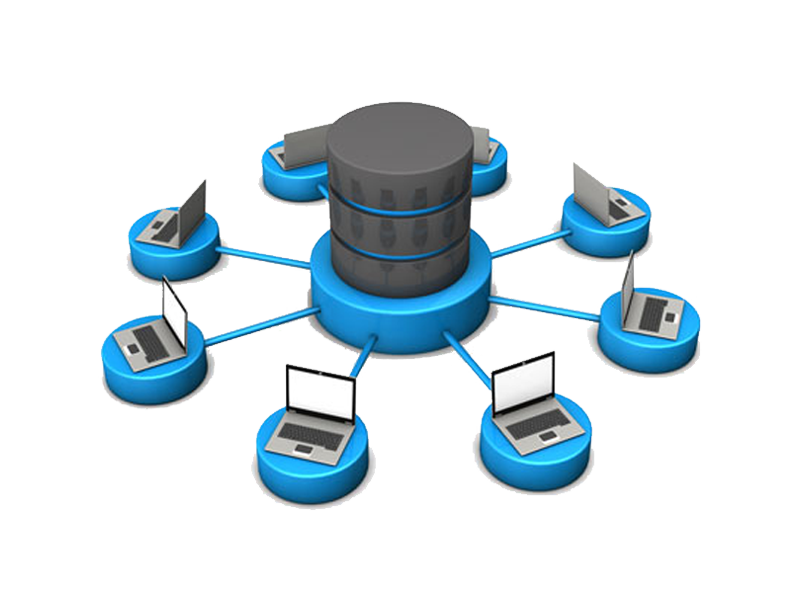
\includegraphics[width=\linewidth]{imagens/banco.png}
%         \label{fig:banco-de-dados}
%     \end{figure}
% \end{columns}
% \end{frame}

\begin{frame}{Modelo Relacional}
    \begin{figure}
        \centering
        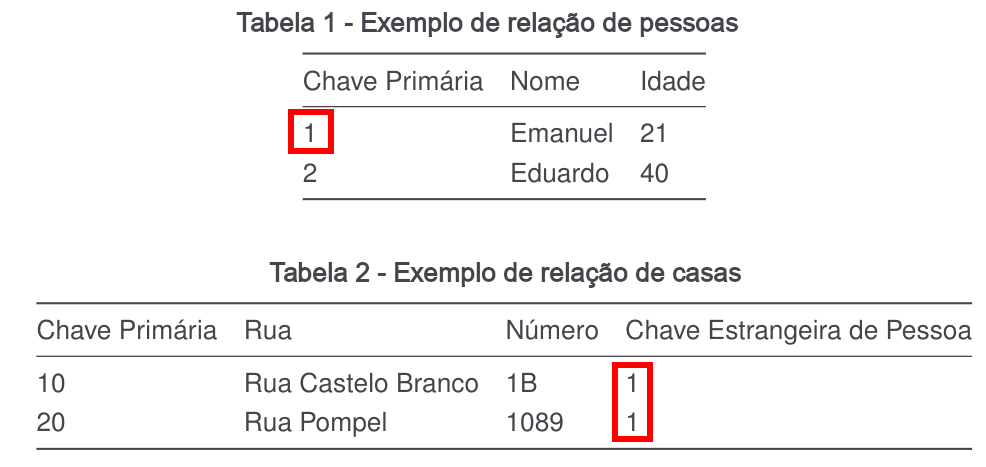
\includegraphics[width=\linewidth]{imagens/relacional.png}
        \label{fig:banco-de-dados-relacional}
    \end{figure}
\end{frame}

\begin{frame}{Normalização}
    \begin{itemize}
        \item Formas normais
        \item Redução de redundância
        \item Otimização de armazenamento
    \end{itemize}
\end{frame}

\begin{frame}{1ª Forma Normal}
\begin{columns}
    \column{0.8\textwidth}
    
    \begin{figure}
        \centering
        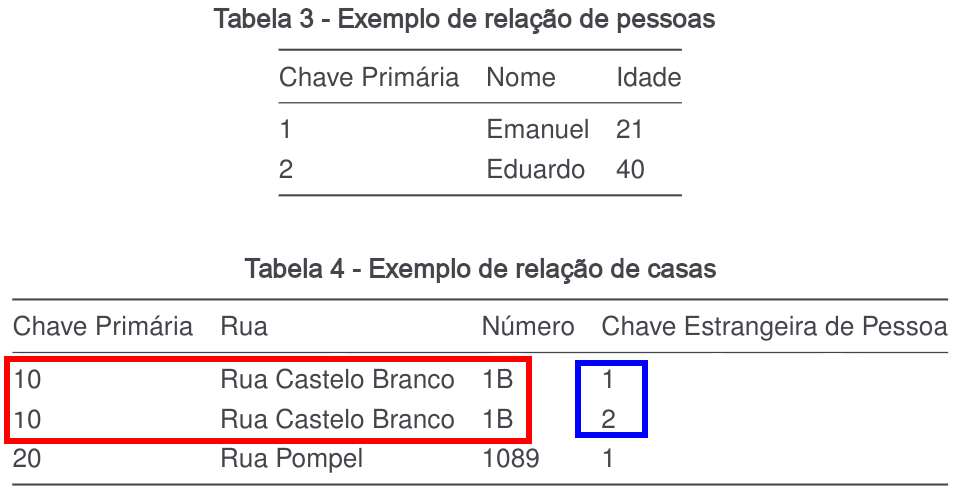
\includegraphics[width=\linewidth]{imagens/1-forma-normal-errado.png}
        \label{fig:1-forma-normal-errado}
    \end{figure}
    
    \column{0.2\textwidth}
    
    \begin{figure}
        \centering
        
\includegraphics[width=\linewidth]{imagens/errado.png}
        \label{fig:1f-errado}
    \end{figure}
\end{columns}
\end{frame}

\begin{frame}{1ª Forma Normal}
\begin{columns}
    \column{0.8\textwidth}
    
    \begin{figure}
        \centering
        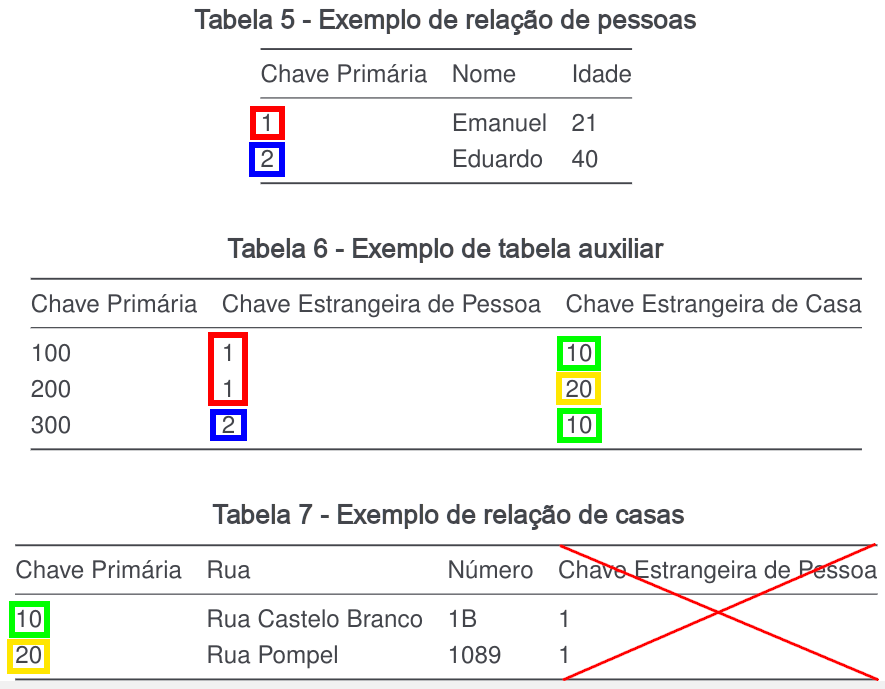
\includegraphics[width=\linewidth]{imagens/1-forma-normal-certo.png}
        \label{fig:1-forma-normal-certo}
    \end{figure}
    
    \column{0.2\textwidth}
    
    \begin{figure}
        \centering
        
\includegraphics[width=\linewidth]{imagens/certo.png}
        \label{fig:1f-certo}
    \end{figure}
\end{columns}
\end{frame}

\begin{frame}{1ª Forma Normal}
    \begin{figure}
        \centering
        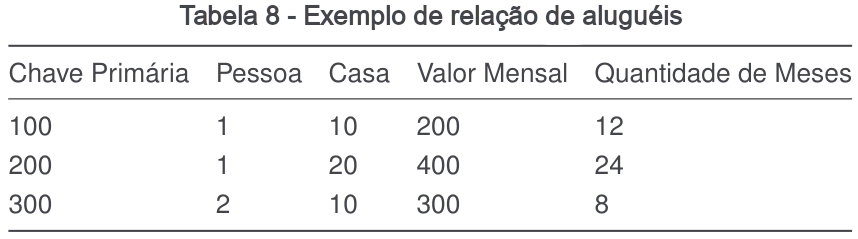
\includegraphics[width=\linewidth]{imagens/tabela-alugueis.png}
        \label{fig:1-forma-normal-certo}
    \end{figure}
\end{frame}

\begin{frame}{2ª Forma Normal}
\begin{columns}
    \column{0.8\textwidth}
    
    \begin{figure}
        \centering
        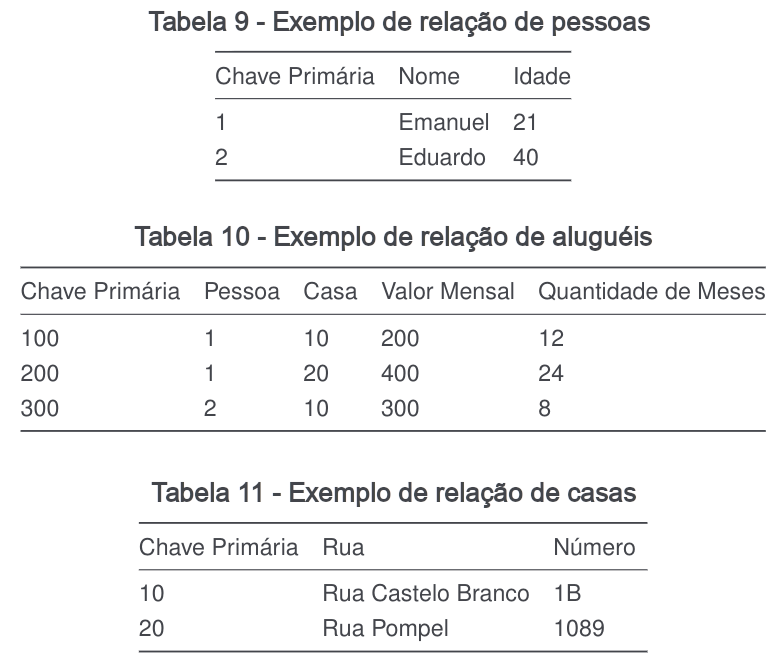
\includegraphics[width=\linewidth]{imagens/2-forma-normal-certo.png}
        \label{fig:2-forma-normal-certo}
    \end{figure}
    
    \column{0.2\textwidth}
    
    \begin{figure}
        \centering
        
\includegraphics[width=\linewidth]{imagens/certo.png}
        \label{fig:2f-certo}
    \end{figure}
\end{columns}
\end{frame}

\begin{frame}{2ª Forma Normal}
    \begin{figure}
        \centering
        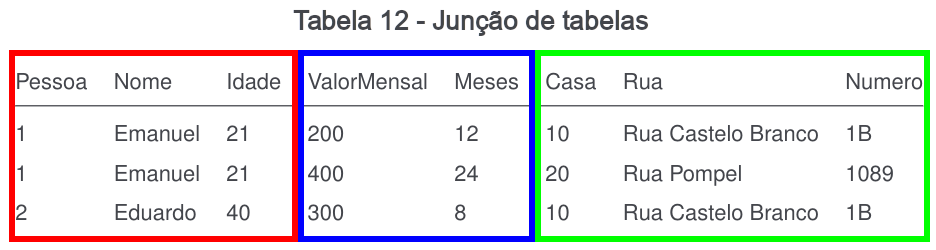
\includegraphics[width=\linewidth]{imagens/2-forma-normal-errado.png}
        \label{fig:2-forma-normal-errado}
    \end{figure}
    \begin{figure}
        \centering
        
\includegraphics[width=0.2\linewidth]{imagens/errado.png}
        \label{fig:2f-errado}
    \end{figure}
\end{frame}

% \begin{frame}{3ª Forma Normal}
%     \justifying{
%         Uma tabela está na Terceira Forma Normal se ela estiver na 2FN e se nenhuma coluna não-chave depender de outra coluna não-chave.
%     }
% \end{frame}

% \begin{frame}{3ª Forma Normal}
% \begin{columns}
%     \column{0.8\textwidth}
    
%     \justifying{
%         Uma tabela está na Terceira Forma Normal se ela estiver na 2FN e se nenhuma coluna não-chave depender de outra coluna não-chave.
%     }
    
%     \vspace{0.5cm}
    
%     \begin{figure}
%         \centering
%         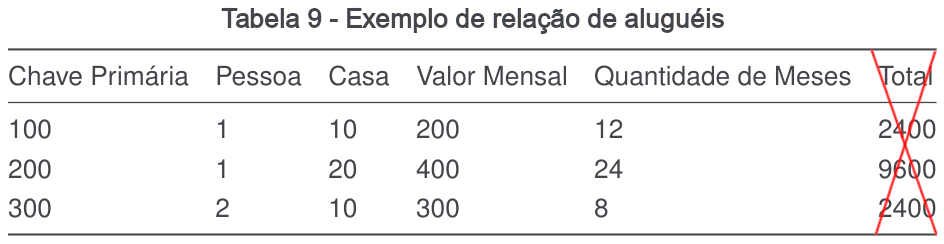
\includegraphics[width=\linewidth]{imagens/3-forma-normal-errado_x.png}
%         \label{fig:3-forma-normal-errado_x}
%     \end{figure}
    
%     \column{0.2\textwidth}
    
%     \begin{figure}
%         \centering
%         
\includegraphics[width=\linewidth]{imagens/errado.png}
%         \label{fig:3f-errado}
%     \end{figure}
% \end{columns}
% \end{frame}

% \begin{frame}{3ª Forma Normal}
% \begin{columns}
%     \column{0.8\textwidth}
    
%     \justifying{
%         Uma tabela está na Terceira Forma Normal se ela estiver na 2FN e se nenhuma coluna não-chave depender de outra coluna não-chave.
%     }
    
%     \vspace{0.5cm}
    
%     \begin{figure}
%         \centering
%         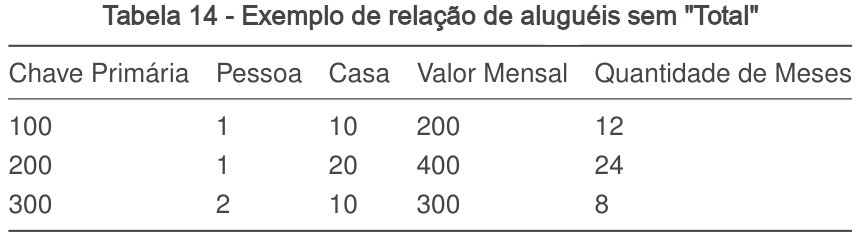
\includegraphics[width=\linewidth]{imagens/3-forma-normal-certo.png}
%         \label{fig:3-forma-normal-certo}
%     \end{figure}
    
%     \column{0.2\textwidth}
    
%     \begin{figure}
%         \centering
%         
\includegraphics[width=\linewidth]{imagens/certo.png}
%         \label{fig:3f-certo}
%     \end{figure}
% \end{columns}
% \end{frame}

\begin{frame}{Desnormalização}
    % \begin{block}{Conceituação}
    %     A desnormalização pode ser definida como o armazenamento de dados em desacordo com as formas normais.
    % \end{block}\pause
    
    % \vspace*{-0.2cm}
    
    \begin{figure}
        \centering
        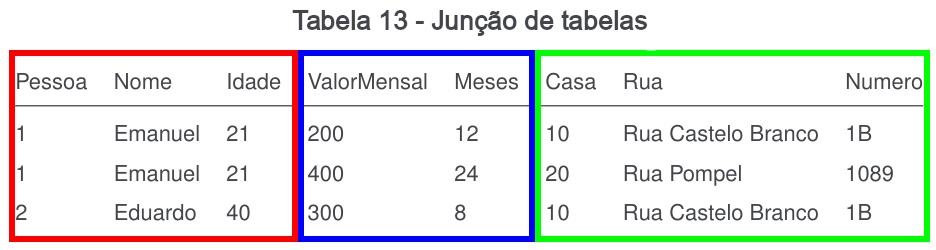
\includegraphics[width=\linewidth]{imagens/tabela-desnormalizada.png}
        \label{fig:tabela-desnormalizada}
    \end{figure}\pause
    
    % \vspace*{-0.6cm}

    \begin{alertblock}{Junção de Tabelas}
        % Existem situações onde tabelas normalizadas precisam ser unidas em uma única tabela desnormalizada através de operações de junção (join).
        Dependendo da aplicação, essa junção \textbf{pode ser cara}.
    \end{alertblock}
\end{frame}

\begin{frame}{NoSQL}
    \begin{block}{Conceituação}
        \justifying{
            Um modelo de Banco de Dados \textbf{NoSQL} é caracterizado pela utilização de um modelo \textbf{não relacional} para o armazenamento de dados
        }
    \end{block}
\end{frame}

\begin{frame}{Por Que Usar o NoSQL?}
    \justifying{
        A alta \textbf{disponibilidade}, a \textbf{baixa tolerância a falhas}, \textbf{confiabilidade de transações}, suporte a dados altamente \textbf{consistentes} e alta \textbf{escalabilidade horizontal}, são requisitos difíceis nos sistemas tradicionais de banco de dados relacional.
    }
    
    \vspace{0.5cm}
    
    \opacitybox{Por isso, os modelos de banco de dados NoSQL tornaram-se uma}\\\opacitybox{tendência emergente de armazenamento de dados}
    
    \vspace{0.5cm}
    
    \flushright{\scriptsize{(DAVOUDIAN AT AL., 2018)}}
\end{frame}

\begin{frame}{Por Que Usar o NoSQL?}
    \justifying{\opacitybox{
        A alta disponibilidade, a baixa tolerância a falhas, confiabilidade de
    }}\\
    \justifying{\opacitybox{
        transações, suporte a dados altamente consistentes e alta escalabil-
    }}\\
    \justifying{\opacitybox{
        idade horizontal, são requisitos difíceis nos sistemas tradicionais de
    }}\\
    \justifying{\opacitybox{
        banco de dados relacional.
    }}
    
    \vspace{0.5cm}
    
    \justifying{
        Por isso, os modelos de banco de dados NoSQL tornaram-se uma tendência emergente de armazenamento de dados
    }
    
    \vspace{0.5cm}
    
    \flushright{\scriptsize{(DAVOUDIAN AT AL., 2018)}}
\end{frame}

% \begin{frame}{Por Que Usar o NoSQL?}
%     \justifying{
%         A alta disponibilidade, a baixa tolerância a falhas, confiabilidade de transações, suporte a dados altamente consistentes e alta escalabilidade horizontal, são requisitos difíceis nos sistemas tradicionais de banco de dados relacional.
%     }
    
%     \vspace{0.5cm}
    
%     \justifying{
%         Por isso, os modelos de banco de dados NoSQL tornaram-se uma tendência emergente de armazenamento de dados
%     }
    
%     \vspace{0.5cm}
    
%     \flushright{\scriptsize{(DAVOUDIAN AT AL., 2018)}}
% \end{frame}

\begin{frame}{MongoDB}
\vspace*{-1.6cm}
\begin{columns}
    \column{0.45\textwidth}

    \begin{figure}
        \centering
        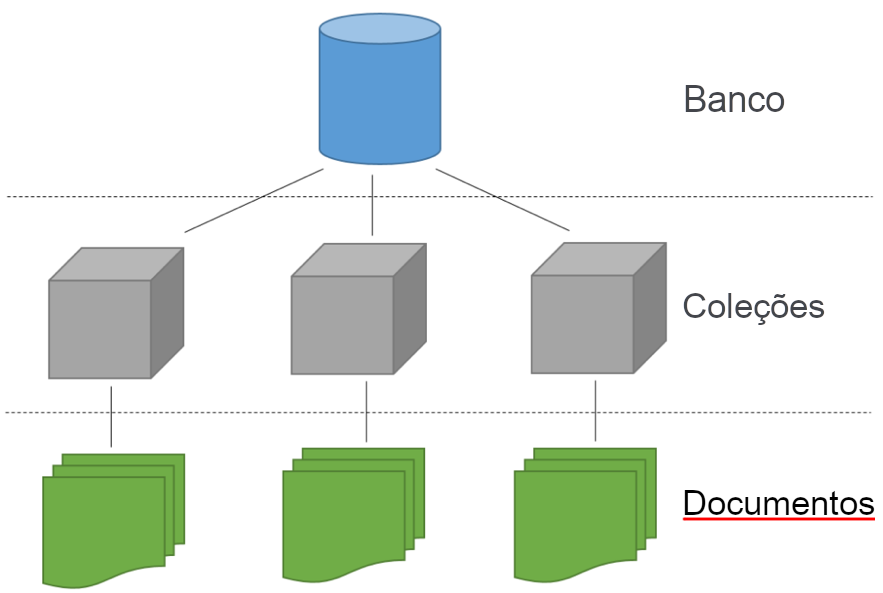
\includegraphics[width=\linewidth]{imagens/mongodb-camadas.png}
        \label{fig:mongodb-camadas}
    \end{figure}
    
    \column{0.66\textwidth}
    
    \begin{figure}
        \centering
        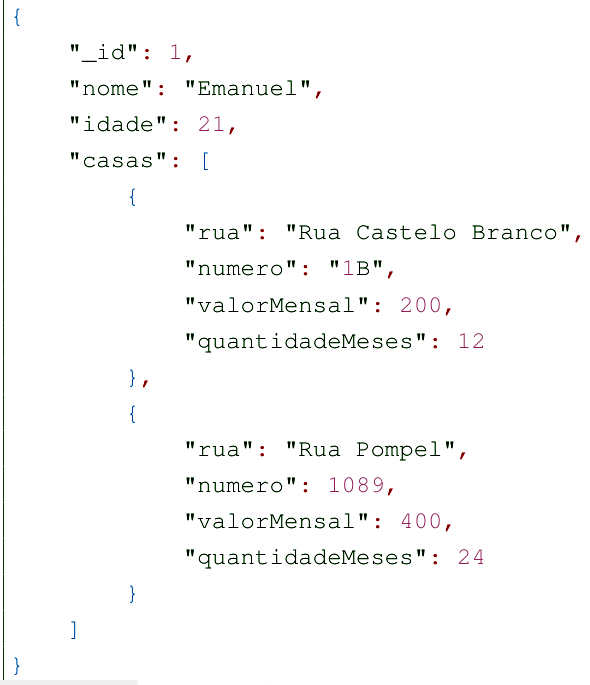
\includegraphics[height=\textheight]{imagens/BJSON_cut.png}
        \label{fig:bjson}
    \end{figure}
\end{columns}
\end{frame}

\section{Problemática}

\begin{frame}
    \begin{figure}
        \centering
        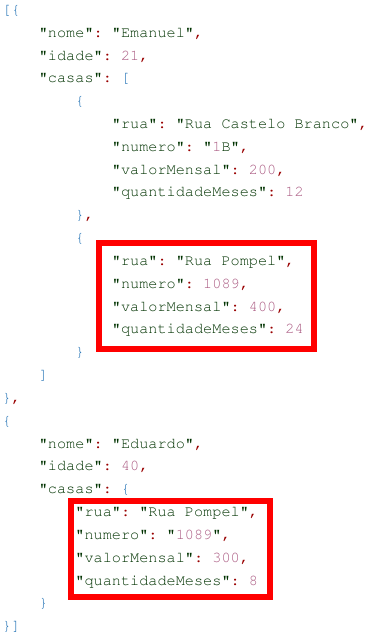
\includegraphics[height=\textheight]{imagens/BJSON-casa-duplicada.png}
        \label{fig:bjson-casa-duplicada}
    \end{figure}
\end{frame}

% \begin{frame}{Normalização com MongoDB}
%     A duplicação de dados, por meio da desnormalização, pode ser problemática. Por causa disso, em determinadas situações, torna-se necessário normalizar os documentos que originalmente estariam desnormalizados
% \end{frame}

\begin{frame}{Normalização com MongoDB}
    \begin{figure}
        \centering
        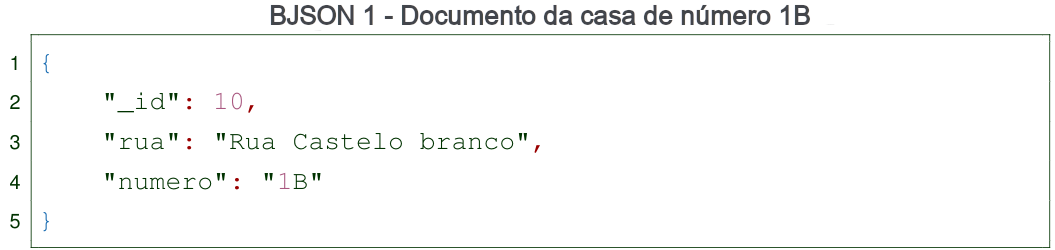
\includegraphics[width=\linewidth]{imagens/casa-1b.png}
        \label{fig:casa-1b}
    \end{figure}
    
    \begin{figure}
        \centering
        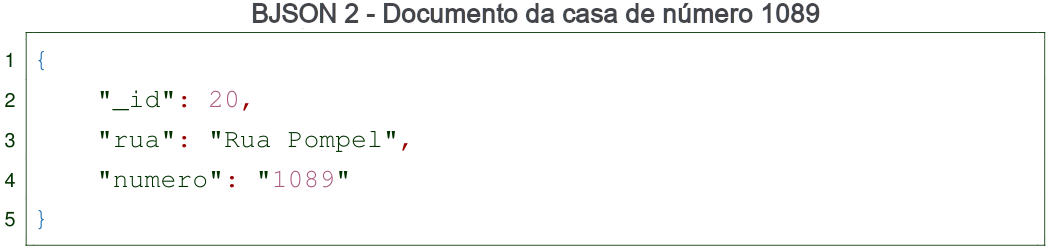
\includegraphics[width=\linewidth]{imagens/casa-1089.png}
        \label{fig:casa-1089}
    \end{figure}
\end{frame}

\begin{frame}{Normalização com MongoDB}
    \begin{figure}
        \centering
        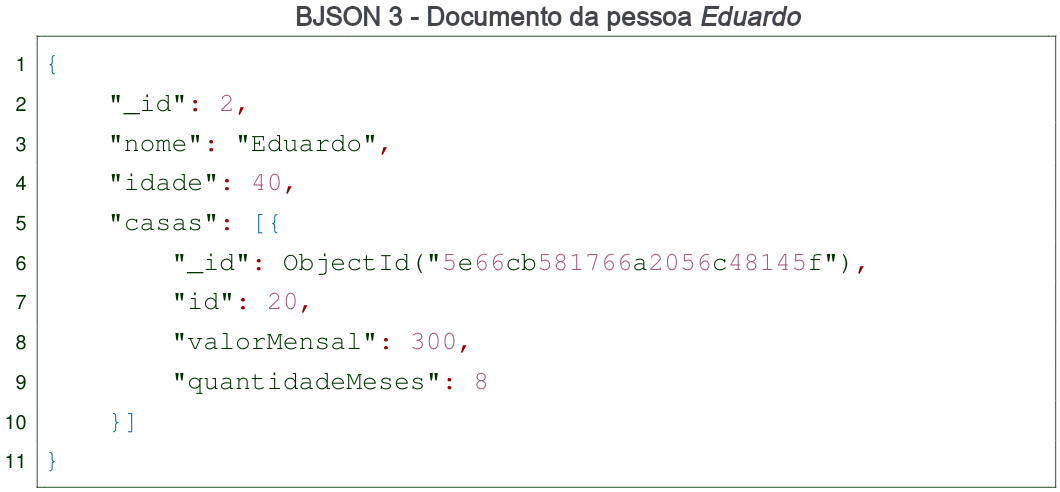
\includegraphics[width=\linewidth]{imagens/pessoa-eduardo.png}
        \label{fig:pessoa-eduardo}
    \end{figure}
\end{frame}

\begin{frame}{Normalização com MongoDB}
    \begin{figure}
        \centering
        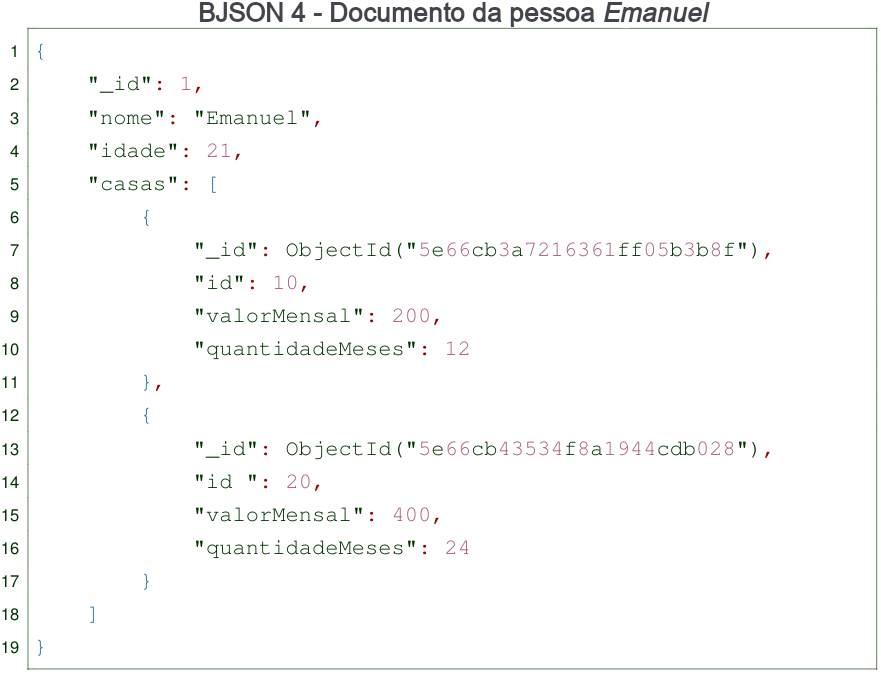
\includegraphics[width=0.8\linewidth]{imagens/pessoa-emanuel.png}
        \label{fig:pessoa-emanuel}
    \end{figure}
\end{frame}

\begin{frame}{Qual é o Problema?}
    \begin{itemize}
        \item \justifying{Com o \textit{MongoDB}, \textbf{operações em dados normalizados}, muitas vezes, são \textbf{menos intuitivas} e \textbf{mais trabalhosas}}
        
        \begin{itemize}
            \item Buscas Sobre Documentos Normalizados
            \item Junção de Documentos
            \item Remoção em Cascata de Documentos
            \item Relação de Dependência Entre os Documentos
            \item Remoção de Identificadores Apontando para Lixo
        \end{itemize}
    \end{itemize}
\end{frame}

\section{Proposta}

\begin{frame}{Objetivos}
    \begin{itemize}
        \item Objetivo Geral
            \begin{itemize}
                \item \justifying{
                    Apresentar o \textbf{\textit{Alpha Restful}} como uma solução capaz de abstrair a implementação de diversas \textbf{funcionalidades} sobre \textbf{dados normalizados} no \textbf{\textit{MongoDB}}
                }
            \end{itemize}
        \item Objetivos Específicos
            \begin{itemize}
                \item \justifying{
                    \textbf{Comparar} algumas ferramentas de mercado (\textbf{\textit{MongoDB}}, \textbf{\textit{Mongoose}}) com o \textit{framework} desenvolvido neste trabalho, através da implementação de algumas funcionalidades
                }
                
                \item \justifying{
                    Mostrar como o \textbf{\textit{Alpha Restful}} se \textbf{sobressai}, em alguns requisitos, em comparação às outras ferramentas utilizadas durante os testes com o \textit{framework} proposto
                }
            \end{itemize}
    \end{itemize}
\end{frame}

\begin{frame}{Tecnologias Utilizadas}
\begin{columns}
    \column{0.5\textwidth}
    
    \begin{figure}
        \centering
        
\includegraphics[width=0.5\linewidth]{imagens/js.jpg}
        \label{fig:js}
    \end{figure}
    
    \begin{figure}
        \centering
        
\includegraphics[width=0.5\linewidth]{imagens/nodejs.jpg}
        \label{fig:nodejs}
    \end{figure}
    
    \column{0.5\textwidth}
    
    \begin{figure}
        \centering
        
\includegraphics[width=0.5\linewidth]{imagens/mongodb-logo.png}
        \label{fig:mongodb}
    \end{figure}
    
    \begin{figure}
        \centering
        
\includegraphics[width=0.9\linewidth]{imagens/mongoose.png}
        \label{fig:mongoose}
    \end{figure}
    
    \vspace{1cm}
\end{columns}
\end{frame}

% \begin{frame}{Como o Alpha Restful Consegue Fazer Essas Otimizações?}
%     \begin{figure}
%         \centering
%         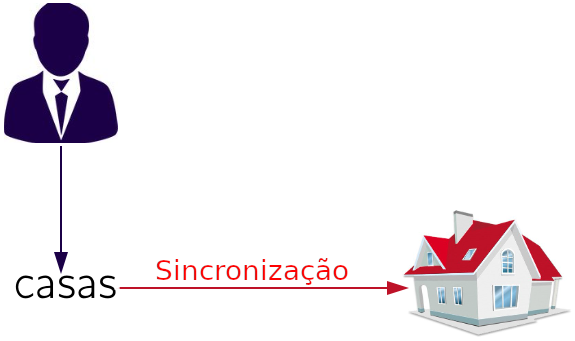
\includegraphics[width=\linewidth]{imagens/sincronizacao-wt.png}
%         \label{fig:sincronizacao}
%     \end{figure}
% \end{frame}

\begin{frame}{Abordagem de Normalização Utilizada pelo \textit{Alpha Restful}}
    \begin{itemize}
        \item Chave estrangeira
        \item Objeto de sincronização (\alert{sync})
        \item Mapeamento de relacionamentos
    \end{itemize}
\end{frame}

\begin{frame}{Modelo Utilizado nas Comparações}
    \begin{figure}
        \centering
        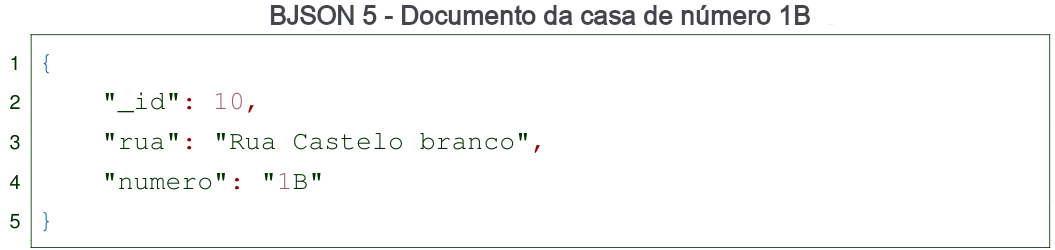
\includegraphics[width=\linewidth]{imagens/casa-1b-2.png}
        \label{fig:metodologia-casa-1b}
    \end{figure}
    
    \begin{figure}
        \centering
        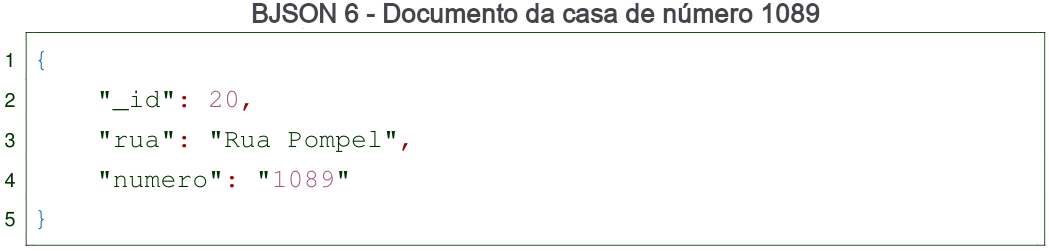
\includegraphics[width=\linewidth]{imagens/casa-1089-2.png}
        \label{fig:metodologia-casa-1089}
    \end{figure}
\end{frame}

\begin{frame}{Modelo Utilizado nas Comparações}
    \begin{figure}
        \centering
        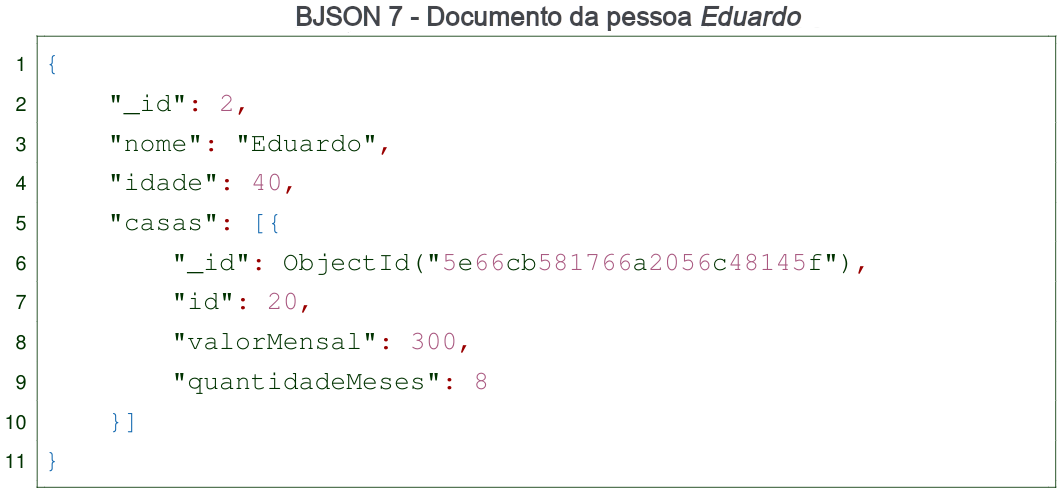
\includegraphics[width=\linewidth]{imagens/pessoa-eduardo-2.png}
        \label{fig:metodologia-pessoa-eduardo}
    \end{figure}
\end{frame}

\begin{frame}{Modelo Utilizado nas Comparações}
    \begin{figure}
        \centering
        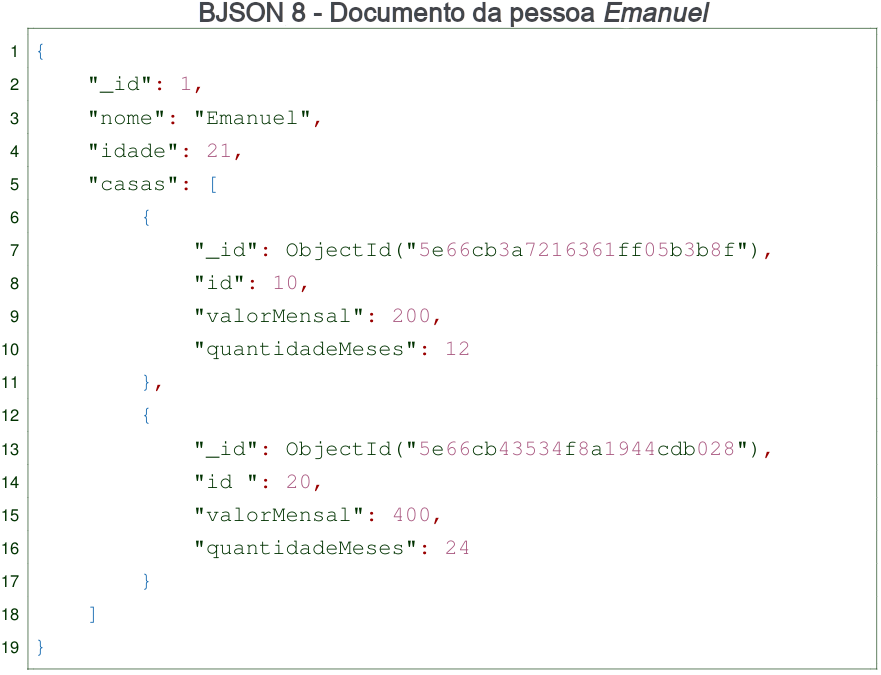
\includegraphics[width=0.8\linewidth]{imagens/pessoa-emanuel-2.png}
        \label{fig:metodologia-pessoa-emanuel}
    \end{figure}
\end{frame}

\section{Resultados}

\begin{frame}{Funcionalidades Otimizadas Pelo \textit{Alpha Restful}}
    \begin{enumerate}
        \item Buscas Sobre Documentos Normalizados
        \item \opacitybox{Junção de Documentos}
        \item \opacitybox{Remoção em Cascata de Documentos}
        \item \opacitybox{Relação de Dependência Entre os Documentos}
        \item \opacitybox{Remoção de Identificadores Apontando para Lixo}
    \end{enumerate}
    
    \vspace{0.7cm}
    
    \begin{block}{Busca Sobre Documentos Normalizados}
        \justifying{
            Como obter todas as casas, na qual existe pelo menos uma pessoa, que essa pessoa possui pelo menos uma casa, que nessa casa possui pelo menos uma pessoa que possui a idade igual a 40 anos?
        }
    \end{block}
\end{frame}

\begin{frame}{Funcionalidades Otimizadas Pelo \textit{Alpha Restful}}
    \begin{enumerate}
        \item Buscas Sobre Documentos Normalizados
            \begin{itemize}
                \item \textcolor{red}{\textit{\$lookup} e \textit{\$math}}
                \item \opacitybox{Forma Manual}
                \item \opacitybox{\textit{Alpha Restful}}
            \end{itemize}
        \item \opacitybox{Junção de Documentos}
            \begin{itemize}
                \item \opacitybox{\textit{populate} (\textit{mongoose})}
                \item \opacitybox{\textit{Alpha Restful}}
            \end{itemize}
        \item \opacitybox{Remoção em Cascata de Documentos}
        \item \opacitybox{Relação de Dependência Entre os Documentos}
        \item \opacitybox{Remoção de Identificadores Apontando para Lixo}
    \end{enumerate}
\end{frame}

\begin{frame}
\vspace*{-0.8cm}
\begin{columns}
    \column{0.4\linewidth}
    
    \begin{figure}
        \centering
        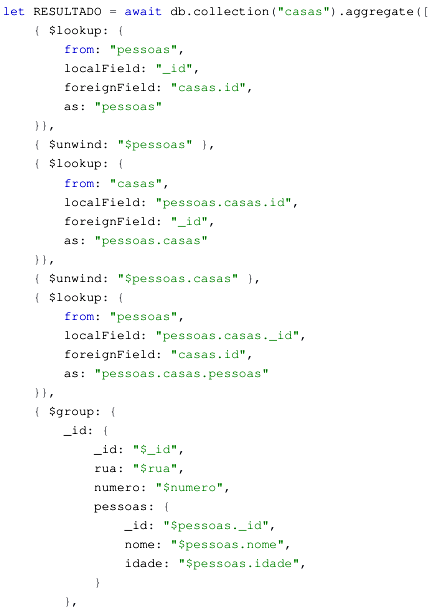
\includegraphics[height=\textheight]{imagens/query-lookup-part-1.png}
        \label{fig:query-lookup-part-1}
    \end{figure}

    \column{0.6\linewidth}
    
    \begin{figure}
        \centering
        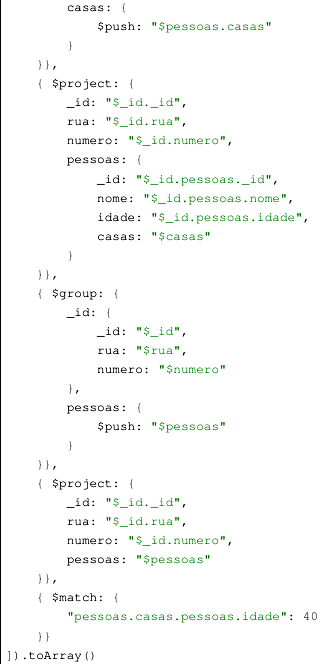
\includegraphics[height=\textheight]{imagens/query-lookup-part-2.png}
        \label{fig:query-lookup-part-2}
    \end{figure}
\end{columns}
\end{frame}

% \begin{frame}
% \vspace*{-0.3cm}
% \begin{columns}
%     \column{0.54\linewidth}

%     \begin{figure}
%         \centering
%         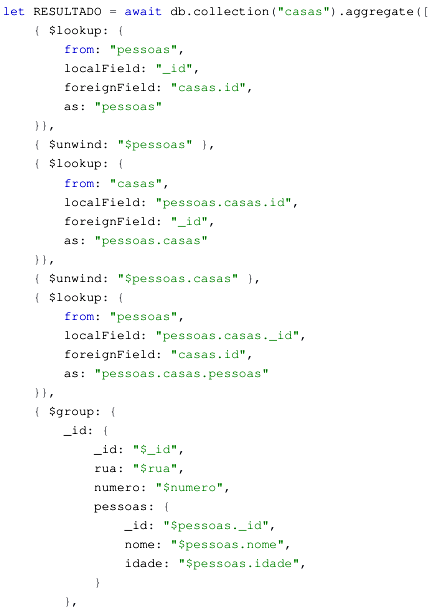
\includegraphics[height=\textheight]{imagens/query-lookup-part-1.png}
%         \label{fig:query-lookup-part-1}
%     \end{figure}
    
%     \column{0.66\linewidth}
    
%     \vspace*{-0.6cm}
%     \begin{figure}
%         \centering
%         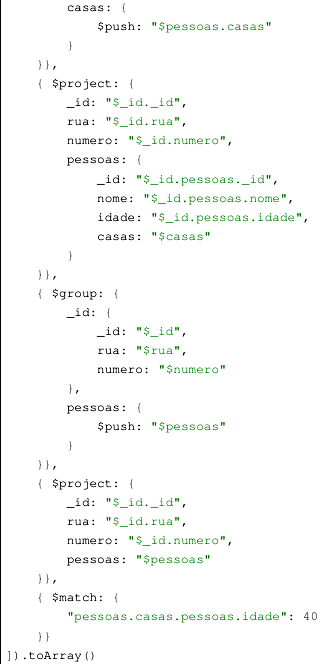
\includegraphics[height=0.95\textheight]{imagens/query-lookup-part-2.png}
%         \label{fig:query-lookup-part-2}
%     \end{figure}
% \end{columns}
% \end{frame}

\begin{frame}{Funcionalidades Otimizadas Pelo \textit{Alpha Restful}}
    \begin{enumerate}
        \item Buscas Sobre Documentos Normalizados
            \begin{itemize}
                \item \opacitybox{\textit{\$lookup} e \textit{\$math}}
                \item \textcolor{red}{Forma Manual}
                \item \opacitybox{\textit{Alpha Restful}}
            \end{itemize}
        \item \opacitybox{Junção de Documentos}
            \begin{itemize}
                \item \opacitybox{\textit{populate} (\textit{mongoose})}
                \item \opacitybox{\textit{Alpha Restful}}
            \end{itemize}
        \item \opacitybox{Remoção em Cascata de Documentos}
        \item \opacitybox{Relação de Dependência Entre os Documentos}
        \item \opacitybox{Remoção de Identificadores Apontando para Lixo}
    \end{enumerate}
\end{frame}

\begin{frame}
    \begin{figure}
        \centering
        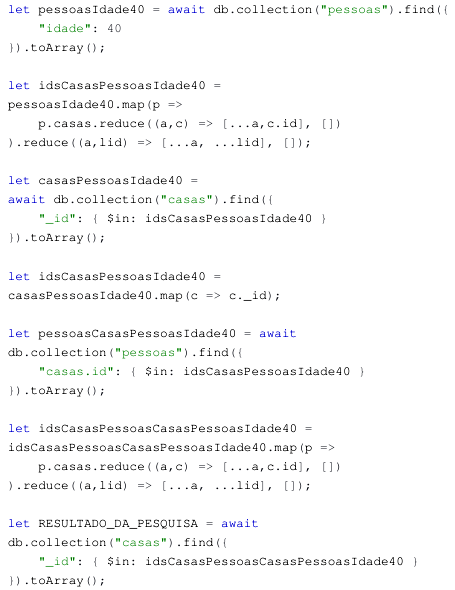
\includegraphics[height=0.98\textheight]{imagens/query-manual.png}
        \label{fig:query-manual}
    \end{figure}
\end{frame}

\begin{frame}{Funcionalidades Otimizadas Pelo \textit{Alpha Restful}}
    \begin{enumerate}
        \item Buscas Sobre Documentos Normalizados
            \begin{itemize}
                \item \opacitybox{\textit{\$lookup} e \textit{\$math}}
                \item \opacitybox{Forma Manual}
                \item \textcolor{red}{\textit{Alpha Restful}}
            \end{itemize}
        \item \opacitybox{Junção de Documentos}
            \begin{itemize}
                \item \opacitybox{\textit{populate} (\textit{mongoose})}
                \item \opacitybox{\textit{Alpha Restful}}
            \end{itemize}
        \item \opacitybox{Remoção em Cascata de Documentos}
        \item \opacitybox{Relação de Dependência Entre os Documentos}
        \item \opacitybox{Remoção de Identificadores Apontando para Lixo}
    \end{enumerate}
\end{frame}

\begin{frame}
    \begin{figure}
        \centering
        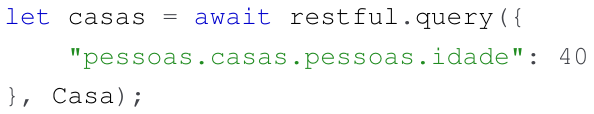
\includegraphics[width=\linewidth]{imagens/query-alpha-restful.png}
        \label{fig:query-alpha-restful}
    \end{figure}
    
    \vspace*{-0.7cm}
    \pause
    
    \begin{figure}
        \centering
        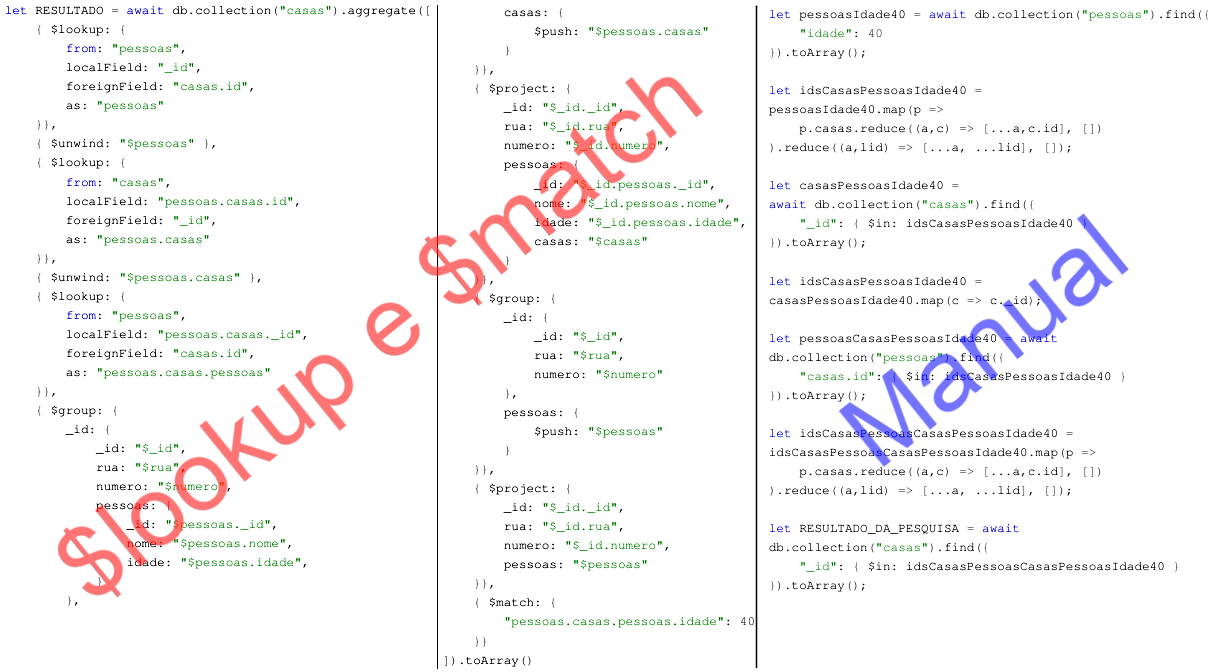
\includegraphics[width=\linewidth]{imagens/compare-others.png}
        \label{fig:compare-others}
    \end{figure}
\end{frame}

\begin{frame}{Funcionalidades Otimizadas Pelo \textit{Alpha Restful}}
    \begin{enumerate}
        \item \opacitybox{Buscas Sobre Documentos Normalizados}
            \begin{itemize}
                \item \opacitybox{\textit{\$lookup} e \textit{\$math}}
                \item \opacitybox{Forma Manual}
                \item \opacitybox{\textit{Alpha Restful}}
            \end{itemize}
        \item Junção de Documentos
            \begin{itemize}
                \item \textcolor{red}{\textit{populate} (\textit{mongoose})}
                \item \opacitybox{\textit{Alpha Restful}}
            \end{itemize}
        \item \opacitybox{Remoção em Cascata de Documentos}
        \item \opacitybox{Relação de Dependência Entre os Documentos}
        \item \opacitybox{Remoção de Identificadores Apontando para Lixo}
    \end{enumerate}
\end{frame}

\begin{frame}
    \begin{figure}
        \centering
        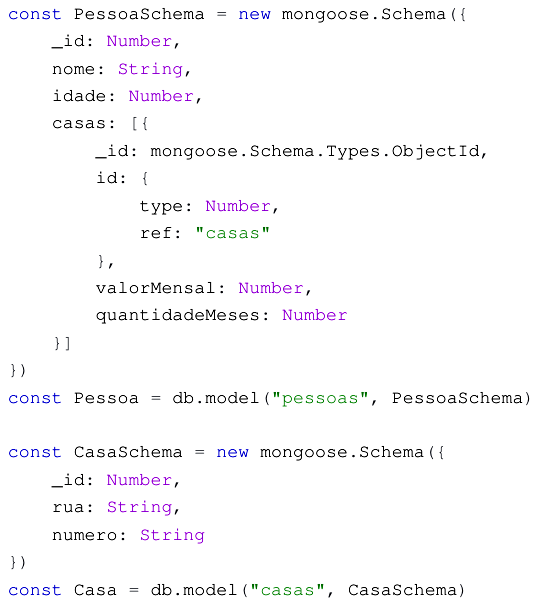
\includegraphics[width=0.6\linewidth]{imagens/schema-mongoose.png}
        \label{fig:schema-mongoose}
    \end{figure}
    
    \begin{figure}
        \centering
        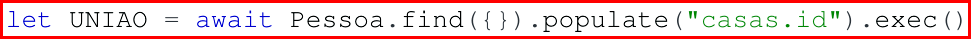
\includegraphics[width=\linewidth]{imagens/populate-mongoose.png}
        \label{fig:populate-mongoose}
    \end{figure}
\end{frame}

\begin{frame}{Funcionalidades Otimizadas Pelo \textit{Alpha Restful}}
    \begin{enumerate}
        \item \opacitybox{Buscas Sobre Documentos Normalizados}
            \begin{itemize}
                \item \opacitybox{\textit{\$lookup} e \textit{\$math}}
                \item \opacitybox{Forma Manual}
                \item \opacitybox{\textit{Alpha Restful}}
            \end{itemize}
        \item Junção de Documentos
            \begin{itemize}
                \item \opacitybox{\textit{populate} (\textit{mongoose})}
                \item \textcolor{red}{\textit{Alpha Restful}}
            \end{itemize}
        \item \opacitybox{Remoção em Cascata de Documentos}
        \item \opacitybox{Relação de Dependência Entre os Documentos}
        \item \opacitybox{Remoção de Identificadores Apontando para Lixo}
    \end{enumerate}
\end{frame}

\begin{frame}
\vspace*{-0.3cm}
\begin{columns}
    \column{0.49\textwidth}

    \begin{figure}
        \centering
        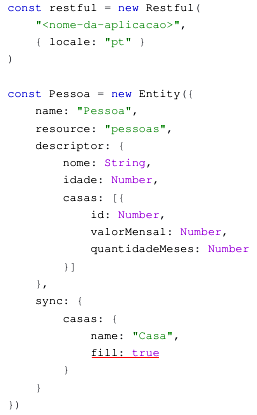
\includegraphics[height=\textheight]{imagens/schema-alpha-restful_part1.png}
        \label{fig:schema-alpha-restful-part1}
    \end{figure}
    
    \column{0.65\textwidth}
    \vspace*{-1.92cm}
    
    \begin{figure}
        \centering
        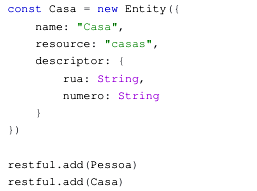
\includegraphics[height=0.5\textheight]{imagens/schema-alpha-restful_part2.png}
        \label{fig:schema-alpha-restful-part2}
    \end{figure}
    
    \vspace*{-0.4cm}
    
    \begin{figure}
        \centering
        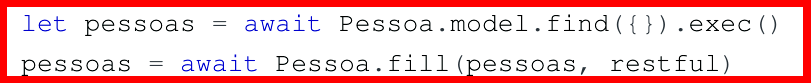
\includegraphics[width= \textwidth]{imagens/fill-alpha-restful.png}
        \label{fig:fill-alpha-restful}
    \end{figure}
    
    \vspace*{-0.5cm}
    
    \begin{itemize}
        \item<2-> \small{Relacionamento Inverso}
        \item<2-> \small{Relacionamento Transitivo}
    \end{itemize}
\end{columns}
\end{frame}

\begin{frame}{Relacionamento Inverso}
    \begin{figure}
        \centering
        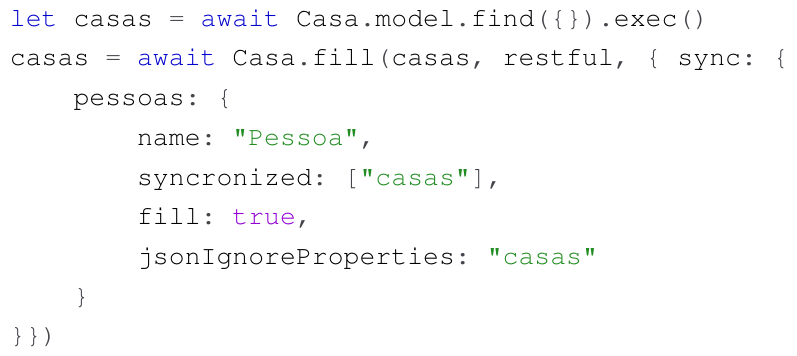
\includegraphics[width=\linewidth]{imagens/relacionamento-inverso-alpha-restful.png}
        \label{fig:relacionamento-inverso-alpha-restful}
    \end{figure}
\end{frame}

\begin{frame}{Relacionamento Transitivo}
    \begin{figure}
        \centering
        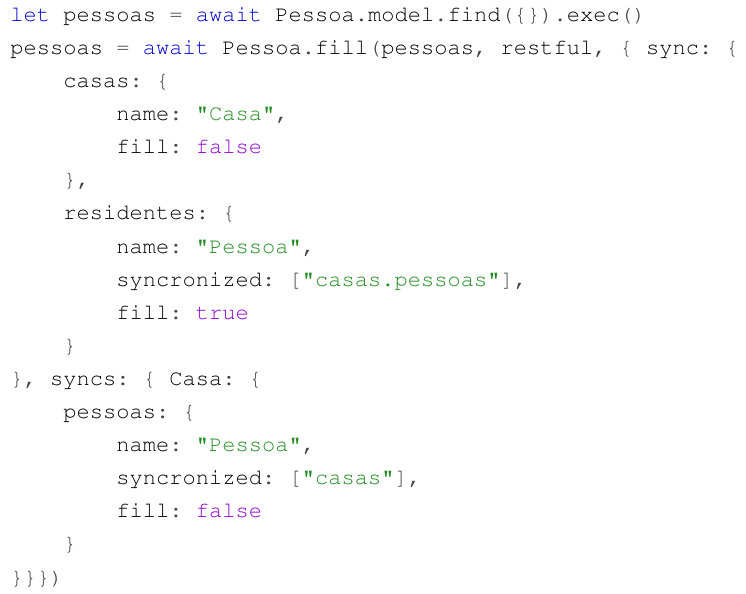
\includegraphics[width=0.88\linewidth]{imagens/relacionamento-inverso-do-relacionamento-inverso-alpha-restful.png}
        \label{fig:relacionamento-inverso-do-relacionamento-inverso-alpha-restful}
    \end{figure}
\end{frame}

\begin{frame}{Funcionalidades Otimizadas Pelo \textit{Alpha Restful}}
    \begin{enumerate}
        \item \opacitybox{Buscas Sobre Documentos Normalizados}
            \begin{itemize}
                \item \opacitybox{\textit{\$lookup} e \textit{\$math}}
                \item \opacitybox{Forma Manual}
                \item \opacitybox{\textit{Alpha Restful}}
            \end{itemize}
        \item \opacitybox{Junção de Documentos}
            \begin{itemize}
                \item \opacitybox{\textit{populate} (\textit{mongoose})}
                \item \opacitybox{\textit{Alpha Restful}}
            \end{itemize}
        \item \textcolor{red}{Remoção em Cascata de Documentos}
        \item \opacitybox{Relação de Dependência Entre os Documentos}
        \item \opacitybox{Remoção de Identificadores Apontando para Lixo}
    \end{enumerate}
\end{frame}

\begin{frame}
    \vspace*{-0.1cm}
    \begin{figure}
        \centering
        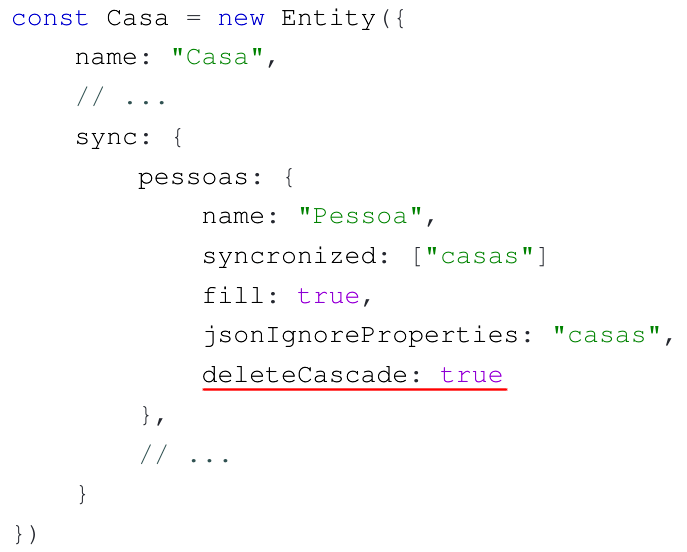
\includegraphics[height=\textheight]{imagens/delete-cascade.png}
        \label{fig:remocao-em-cascata}
    \end{figure}
\end{frame}

\begin{frame}{Funcionalidades Otimizadas Pelo \textit{Alpha Restful}}
    \begin{enumerate}
        \item \opacitybox{Buscas Sobre Documentos Normalizados}
            \begin{itemize}
                \item \opacitybox{\textit{\$lookup} e \textit{\$math}}
                \item \opacitybox{Forma Manual}
                \item \opacitybox{\textit{Alpha Restful}}
            \end{itemize}
        \item \opacitybox{Junção de Documentos}
            \begin{itemize}
                \item \opacitybox{\textit{populate} (\textit{mongoose})}
                \item \opacitybox{\textit{Alpha Restful}}
            \end{itemize}
        \item \opacitybox{Remoção em Cascata de Documentos}
        \item \textcolor{red}{Relação de Dependência Entre os Documentos}
        \item \opacitybox{Remoção de Identificadores Apontando para Lixo}
    \end{enumerate}
\end{frame}

\begin{frame}
    % \vspace*{-0.7cm}
    \begin{figure}
        \centering
        \includegraphics[width=\linewidth]{imagens/relacao-de-dependencia.png}
        \label{fig:relacao-de-dependencia}
    \end{figure}
\end{frame}

\begin{frame}{Funcionalidades Otimizadas Pelo \textit{Alpha Restful}}
    \begin{enumerate}
        \item \opacitybox{Buscas Sobre Documentos Normalizados}
            \begin{itemize}
                \item \opacitybox{\textit{\$lookup} e \textit{\$math}}
                \item \opacitybox{Forma Manual}
                \item \opacitybox{\textit{Alpha Restful}}
            \end{itemize}
        \item \opacitybox{Junção de Documentos}
            \begin{itemize}
                \item \opacitybox{\textit{populate} (\textit{mongoose})}
                \item \opacitybox{\textit{Alpha Restful}}
            \end{itemize}
        \item \opacitybox{Remoção em Cascata de Documentos}
        \item \opacitybox{Relação de Dependência Entre os Documentos}
        \item \textcolor{red}{Remoção de Identificadores Apontando para Lixo}
    \end{enumerate}
\end{frame}

\begin{frame}{Código a ser Executado Antes de Remover Casa}
    \begin{figure}
        \centering
        \includegraphics[width=\linewidth]{imagens/antes-de-remover.png}
        \label{fig:antes-de-remover}
    \end{figure}
\end{frame}

\section{Conclusões}

\begin{frame}{Conclusões}
    \begin{itemize}
        \item \justifying{
            O \textbf{\textit{Alpha Restful}} \textbf{facilita} e \textbf{automatiza} a implementação de diversas funcionalidades sobre dados normalizados que, por sua vez, são mais simples e intuitivas, em \textbf{comparação} com as ferramentas disponibilizadas pelo \textbf{\textit{MongoDB}} e \textbf{\textit{Mongoose}}
        }
        
        \item \justifying{
            A facilidade, disponibilizada pelo \textbf{\textit{Alpha Restful}}, de manipular dados normalizados no \textit{MongoDB}, possibilita que a aplicação possa \textbf{escolher a melhor abordagem} (normalização ou desnormalização), para cada caso específico, \textbf{sem um grande aumento na complexidade} do desenvolvimento
        }
    \end{itemize}
\end{frame}

\begin{frame}{Trabalhos Futuros}
    \begin{itemize}
        % \item \justifying{
        %     Implementar algo equivalente às \textit{views} do SQL. Com isso, na modelagem das entidades, torna-se possível definir atributos que serão resultados de uma sub-consulta feita em tempo de execução
        % }
        
        \item \justifying{
            Implementar sub-consultas a serem usados em pesquisas, junções de documentos e na própria modelagem das entidades
        }
        
        \item \justifying{
            Disponibilizar interfaces para que outros bancos de dados NoSQL possam ser usados pelo \textit{Alpha Restful}
        }
        
        \item \justifying{
            Analisar a performance do \textit{framework}, a fim de que uma nova versão estável possa ser lançada
        }
    \end{itemize}
\end{frame}

\rmsection

\begingroup
\setbeamertemplate{headline}{}
\setbeamertemplate{navigation symbols}{}
\frame{
    \vspace*{-0.5cm}
    \centering{\alert{Obrigado!}}
    \titlepage
} % Cria página de título final
\endgroup

\end{document}
